%\documentclass[a4paper]{book}
%\usepackage{mcmd}

%\begin{document}

\section{msortf - Sort Records\label{sect:msortf}}
\index{msortf@msortf}
Sort records according to the field defined at \verb|f=| parameter.\\
This commands uses quicksort algorithm and it is not a stable sort (original order is retained for rows with same key value).  \\

\subsection*{Format}
\verb|msortf f= [pways=] [maxlines=] [blocks=] [threadCnt=] [-noflg]|
\hyperref[sect:option_i]{[i=]}
\hyperref[sect:option_o]{[o=]}
\hyperref[sect:option_assert_diffSize]{[-assert\_diffSize]}
\hyperref[sect:option_nfn]{[-nfn]} 
\hyperref[sect:option_nfno]{[-nfno]}  
\hyperref[sect:option_x]{[-x]}
\hyperref[sect:option_q]{[-q]}
\hyperref[sect:option_tmpPath]{[tmpPath=]} 
\verb|[--help]|
\verb|[--helpl]|
\verb|[--version]|\\
\renewcommand{\figurename}{Figure }

\subsection*{Parameters}
\begin{table}[htbp]
%\begin{center}
{\small
\begin{tabular}{ll}
\verb|f=|     & Specify the column name where record values will be sorted accordingly. \\
             	& Four types of sequence order can be specified namely numeric, string, ascending, descending. \\
       		    & Specify \verb|%n| after the field name, followed by \verb|n| or \verb|r|. \\
		          & Character string ascending order:\verb|field name| (\verb|%| is not specified), character string descending order:\verb|f=field%r|, \\
		          & numeric ascending order:\verb|f=field%n|, numeric descending order:\verb|f=field%nr|.\\
\verb|-noflg| & Do not attach sorting marks (\verb |%0,%0n| etc.) to the output CSV header.\\
\end{tabular} 
}
\end{table} 

\subsection*{Remarks}
\begin{enumerate}
\item Character string fields specified at \verb|k=| may not be sorted correct when \verb|%n| is specified. 
\item When \verb|k=| is not specified, specify the files in merging order at \verb|i=| (same as \hyperref[sect:mcat]{mcat}).
\item When key field include NULL values, NULL value is treated as a value less than any value. 
\item Field names of all input data specified at \verb|i=| is assumed to have the same field names, whereas \verb|mcat| has more flexibility in field names. 
\end{enumerate}



\subsection*{Examples}
\subsubsection*{Example 1: Basic example}

Sort by \verb|item| and \verb|date|.


\begin{Verbatim}[baselinestretch=0.7,frame=single]
$ more dat1.csv
item,date,quantity,price
B,20081201,4,40
A,20081201,10,200
A,20081201,10,100
B,20081203,5,50
B,20081201,2,500
A,20081201,3,300
$ msortf f=item,date i=dat1.csv o=rsl1.csv
#END# kgsortf f=item,date i=dat1.csv o=rsl1.csv
$ more rsl1.csv
item%0,date%1,quantity,price
A,20081201,10,200
A,20081201,10,100
A,20081201,3,300
B,20081201,4,40
B,20081201,2,500
B,20081203,5,50
\end{Verbatim}
\subsubsection*{Example 2: Sort by quantity in descending order and price in ascending order.}



\begin{Verbatim}[baselinestretch=0.7,frame=single]
$ msortf f=quantity%nr,price%n i=dat1.csv o=rsl2.csv
#END# kgsortf f=quantity%nr,price%n i=dat1.csv o=rsl2.csv
$ more rsl2.csv
item,date,quantity%0nr,price%1n
A,20081201,10,100
A,20081201,10,200
B,20081203,5,50
B,20081201,4,40
A,20081201,3,300
B,20081201,2,500
\end{Verbatim}


\subsection*{Advanced parameters}
\begin{table}[htbp]
%\begin{center}
{\small
\begin{tabular}{ll}
\verb|pways=|    & Merge multiple files simultaneously ([2-100]:default 32) [Optional]\\
                 & Specify  number of files to merge at a time while sorting multiple files. \\
\verb|blocks=|   & Number of buffer block ([1-1000]: default 100 1blk=400KB) [Optional]\\
                 & Specify memory size limit in the block size when sorting in memory.\\
                 & Maximum size for 1 block is × 4. Default = 400KB. \\
\verb|maxlines=| & Row fetch limit of memory sort ([100-10,000,000]: 500,000 defaults) [Optional]\\
                 & Specify the maximum number of records sorted at once in memory.\\
                 & Set -block limit and -maxlines limit depending on the average size of record in the data.\\
\verb|threadCnt=|& Number of threads to use when sorting in memory ([1-50] Default: 8) [Optional]\\
                 & Specify the number of threads for sorting through multi-threading function. \\
\end{tabular} 
}
\end{table} 

\subsection*{Notes on sorting order of CSV special characters}
msortf interprets and sorts CSV special characters (e.g. comma and double quotes) differently than the sort command in UNIX. The data fields/columns are separated by comma character. For example, the values in the first column (f1) from the first row onwards are represented by the following ASCII characters: 
a -> (0x61)
null -> (0x00)
space -> (0x20)
+ -> (0x2b)
- -> (0x2d)
, -> (0x2c) 
" -> (0x22)
Comma and double quotes is treated as special characters in CSV is enclosed in double quotes. 
For ease of illustration, "x" is populated in the second column f2 for all records as follows. \\

\begin{verbatim}[baselinestretch=0.7,frame=single,fontsize=\small]
------------------------------------------------
f1,f2
a,x
,x
 ,x
+,x
-,x
",",x
"""",x
------------------------------------------------
\end{verbatim}

The statement \verb|"msortf f=f1"| sorts the data as follows.  The sort order for CSV format special characters (null, space, double quotation, +, comma,-, a) is explained. 

\begin{verbatim}
------------------------------------------------
f1,f2
,x
 ,x
"""",x
+,x
",",x
-,x
a,x
------------------------------------------------
\end{verbatim}

\subsection*{Benchmark Test}
The benchmark test described here shows the performance of msort and msortf. 
The input data consist of 6 fields and all data values are uniform random numbers. \\

\begin{verbatim}
------------------------------------------------
key,fld1,fld2,fld3,fld4,fldn
95547922,162,159,192,118,74
81438069,138,157,155,122,58
26885062,129,199,133,198,75
32651684,180,107,123,170,-14
10245631,164,103,159,154,-63
15145156,182,191,175,107,-60
29254245,188,185,129,124,5
85423170,116,164,175,113,57
55155879,105,163,195,167,25
66997216,195,139,195,113,39
.
.
------------------------------------------------
\end{verbatim}

\subsection*{Compare number of key types and values}
The sample data size is 1 million, the following table shows the results according to variation in types of key values at 2,10,100,1000,10000.
Data in the "random number" column is generated using the maximum limit of the random number as key. 
Data is sorted according to the values in "random number ascending / descending order" column before the benchmark test. 
The comparison table shows the processing results of msort, MUSASHI xtsort command, and UNIX sort command against the msortf command.
The sort command sort one or more sort keys extracted from each line of input, whereas "sort -k1" sorts data on the first column. 
The last 3 rows of the table show the result of  msortf, xtsort and sort sorted on numeric value stored in the first key field.
※ Input data size: about 28MB.\\
※ Unit: seconds. Measurement in real time from beginning to end of program using the time command. \\
※ Environment: iMac, Mac OS X 10.5 Leopard, 2.8GHz Intel Core 2 Duo, 4GB memory \\

%\begin{table}[hbt]
\begin{center}
\caption{Comparison of types of key values and its condition among various sort commands}
\begin{tabular}{clrrrrrrrr}
\hline
No. & Command & 2 Types & 10 Types & 100 Types & 1000 Types & 10000 Types & Rand & Rand Asc & Rand Desc \\
\hline
(1)&msortf f=key&0.29&0.33&0.37&0.40&0.43&0.50&0.29&0.28 \\
(2)&xtsort -k key&1.25&1.24&1.22&1.20&1.19&1.12&0.85&1.00 \\
(3)&sort -k1&16.96&16.63&16.05&15.56&15.08&13.68&6.85&7.13 \\
\hline
(4)&msortf f=key\%n&0.46&0.56&0.65&0.72&0.79&1.02&0.59&0.59 \\
(5)&xtsort -k key\%n&2.52&2.72&2.96&3.16&3.21&3.22&2.31&2.32 \\
(6)&sort -k1 -n&16.65&14.52&11.54&8.56&5.71&0.95&0.33&0.36 \\
\hline
\end{tabular}
\end{center}
\end{table}

\begin{table}[hbt]
\begin{center}
\caption{Comparison of types of key values and its condition among various sort commands}
\begin{tabular}{clrrrrrrrr}
\hline
No. & Command & 2 Types & 10 Types & 100 Types & 1000 Types & 10000 Types & Rand & Rand Asc & Rand Desc \\
\hline
(1)&msortf f=key&0.29&0.33&0.37&0.40&0.43&0.50&0.29&0.28 \\
(2)&xtsort -k key&1.25&1.24&1.22&1.20&1.19&1.12&0.85&1.00 \\
(3)&sort -k1&16.96&16.63&16.05&15.56&15.08&13.68&6.85&7.13 \\
\hline
(4)&msortf f=key\%n&0.46&0.56&0.65&0.72&0.79&1.02&0.59&0.59 \\
(5)&xtsort -k key\%n&2.52&2.72&2.96&3.16&3.21&3.22&2.31&2.32 \\
(6)&sort -k1 -n&16.65&14.52&11.54&8.56&5.71&0.95&0.33&0.36 \\
\hline
\end{tabular}
\end{center}
\end{table}


%The graph of item (1) and (2) in the above table is shown below. 
\begin{figure}[hbt]
\begin{center}
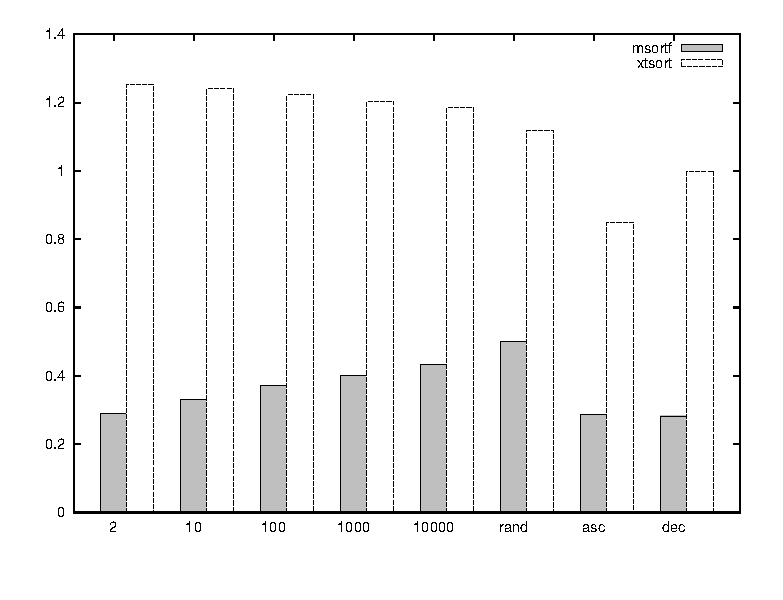
\includegraphics[scale=.8]{figure/msortf/key.eps}
\end{center}
\vspace{10 mm}
\caption{Compare sort results on character strings with msort, msortf, xtsort on various key types. (x-axis: number of the key types, y-axis: seconds)\label{fig:msortf:bench1}}
\end{figure}

%The graph of item (4) and (5) in the above table is shown below. 
\begin{figure}[hbt]
\begin{center}
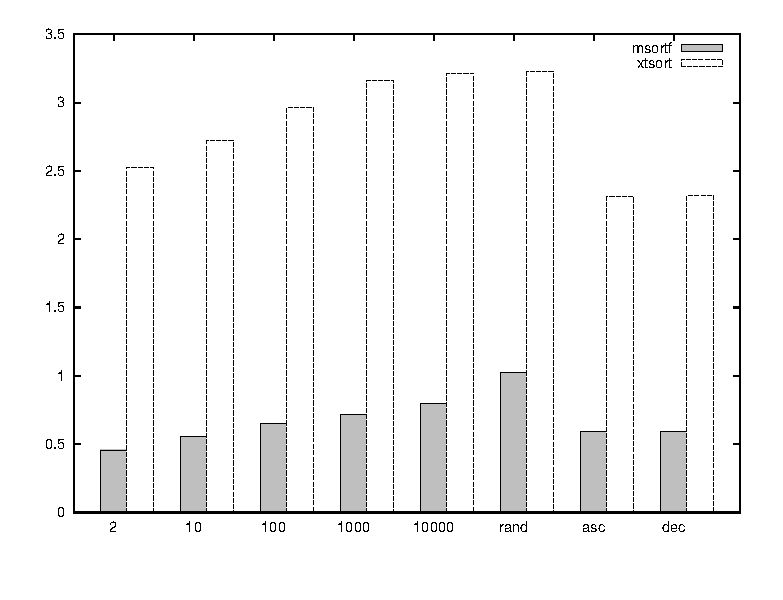
\includegraphics[scale=.8]{figure/msortf/num.eps}
\end{center}
\vspace{10 mm}
\caption{Compare sort results on numerical values with msortf,xtsort on various key types (x-axis: number of key types, y-axis: seconds)\label{fig:msortf:bench2}}
\end{figure}

msortf is 2 to 5 times faster than xtsort. In relation to sort, it can be more than ten times faster depending on the conditions. This command uses the exactly the same quick sort algorithm as in MUSASHI, however, in MCMD multi-threading is used for the parallel processing of sort in separate threads. The impact of the difference is shown. 

Next, the experiment shows the change in speed of character string sorting from 1 million records to 10 million records given the number of key types is set as 100 and the maximum value. 
The comparison of the two commands msortf and xtsort is shown in Figure \ref{fig:msortf:bench3}, \ref{fig:msortf:bench4}. 


%As shown in the benchmark test, msort is 1.5 times faster than MUSASHI xtsort. Even though both commands uses the same quicksort algorithm, msort leverages on multi-threaded sort processing using kgmod which runs 1.5 times faster. 
%msort performs better than msortf on data with irregular keys that is sorted beforehand, as sorting is done by line without dividing the data. Thus, small variation in key types for the first item makes it difficult for comparison as the correlation magnitude has not been established.  The need for comparison created a higher overhead. 
%In addition, the msort command process faster than msortf on data with multiple columns.  However, using msort to sort the key field of input data for other commands may yield different results if the command is executed incorrectly. For more information, refer to msort command. \\

%The results also show that msortf is two times more efficient than xtsort in sorting numeric fields.
%Next, the sorting speed is compared amongst msortf, msort, and xtsort on data with a sample size of 10 million with 2 to 100 different key values. The results are shown as follows: \\

\begin{figure}[hbt]
\begin{center}
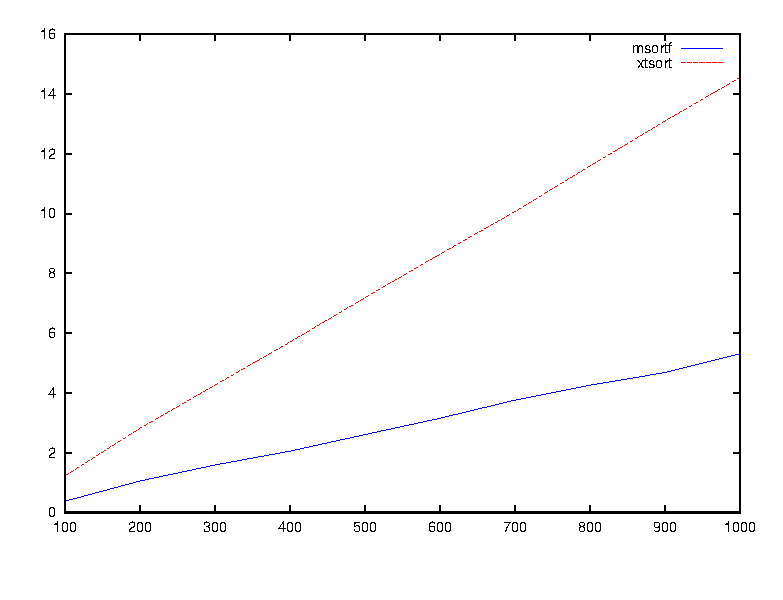
\includegraphics[scale=.8]{figure/msortf/line_100.eps}
\end{center}
\vspace{10 mm}
\caption{Sorting results with 100 key types (x-axis: number of records, y-axis: seconds)\label{fig:msortf:bench3}}
\end{figure}

\begin{figure}[hbt]
\begin{center}
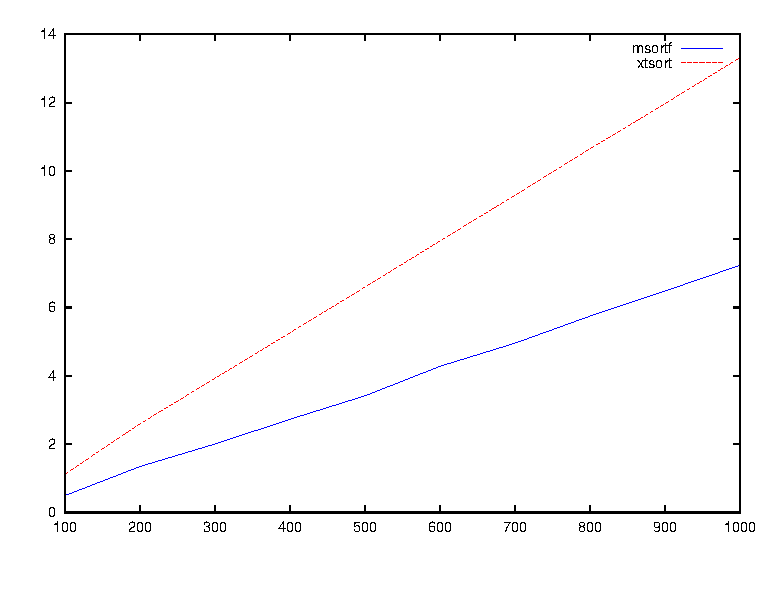
\includegraphics[scale=.8]{figure/msortf/line_rand.eps}
\end{center}
\vspace{10 mm}
\caption{Sorting results with different key types using random number (maximum) (x-axis: number of records, y-axis: seconds)\label{fig:msortf:bench4}}
\end{figure}

\subsection*{Related Command}


%\end{document}
